\cleardoublepage
\section{MTU Discovery}

Netzwerk Pakete beinhalten typischerweise mehrere Netzwerkprotokolle. Diese Protokolle sind in Layern angeordnet und haben klar definierte Schnittstellen. Dadurch sind sie grösstenteils unabhängig voneinander und können ausgetauscht werden. Bei der Kommunikation mit einem Webserver hat man zum Beispiel den folgenden Aufbau\footnotemark[1]. HTTP über TCP/IP über Ethernet.

\begin{figure}[H]
    \begin{center}
        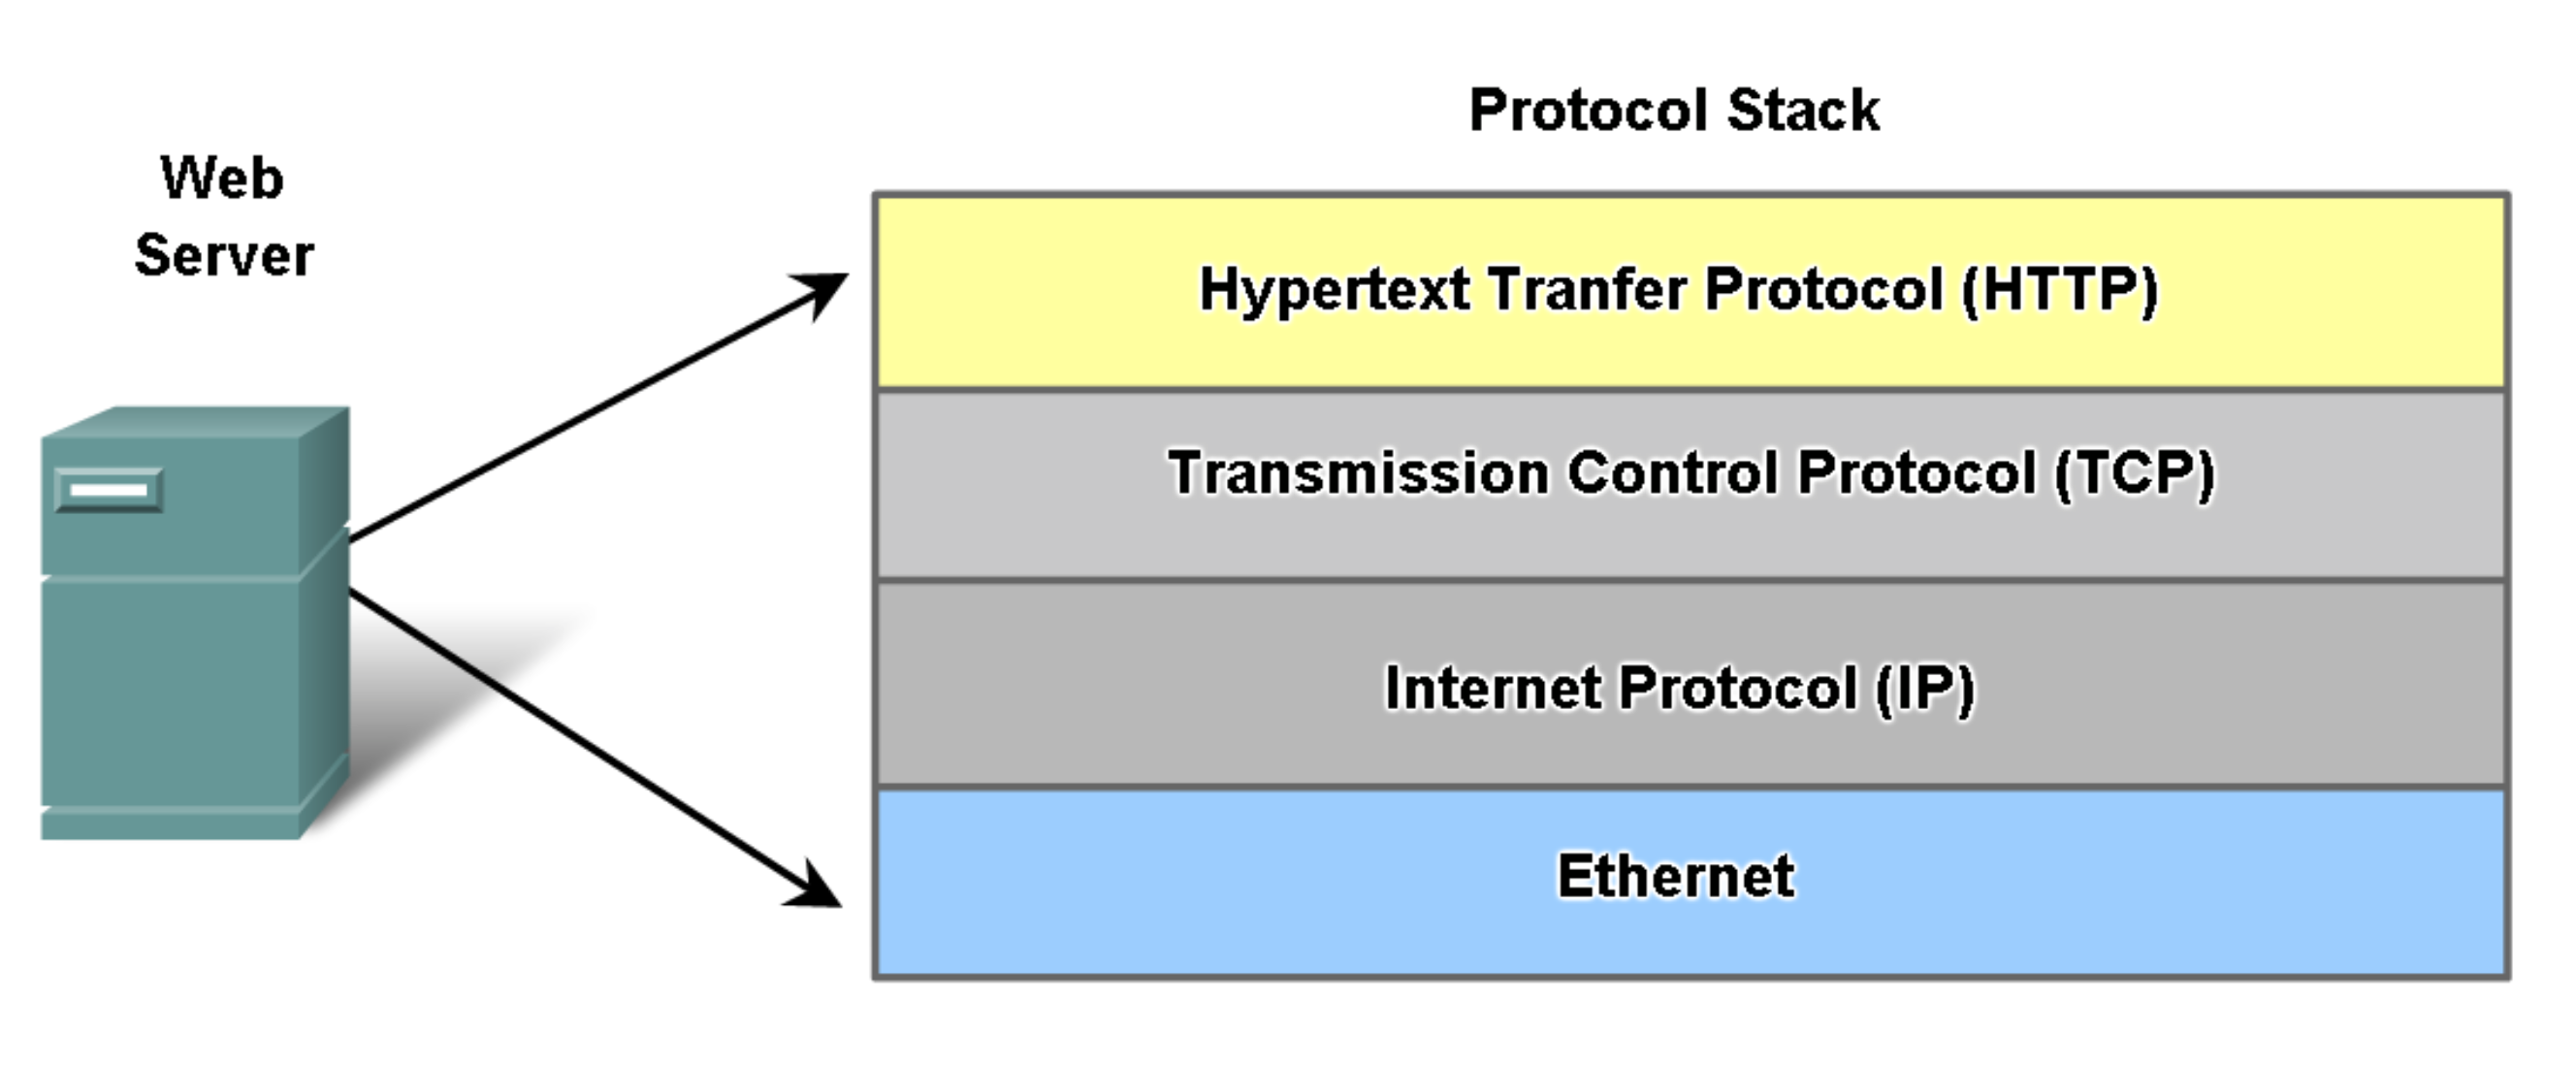
\includegraphics[trim=1 0 0 0,clip,width=\textwidth]{mainpart/analyse/img/HTTP_Stack}
    \end{center}
    \caption{Protokoll Stack eines typischen HTTP Requests}
\end{figure}

\footnotetext[1]{Bild: HSR Vorlesung CN1 - Steffen/Stettler, 29.07.2014, 1-Grundlagen.ppt}

Man ist aber nicht an genau diese Struktur gebunden. Man könnte zum Beispiel den Ethernet Layer durch einen anderen Layer austauschen und die restlichen Protokolle so belassen.

Um das Zusammenspiel der unterschiedlichen Netzwerk Layern besser zu veranschaulichen wurde das \ac{OSI}-Modell entwickelt. Das OSI Modell besteht aus 7 Layern die jeweils unterschiedliche Aufgaben haben. Protokolle die im gleichen \ac{OSI}-Layer mit klaren Schnittstellen definiert wurde sind einfach austauschbar.

\begin{figure}[H]
    \begin{center}
        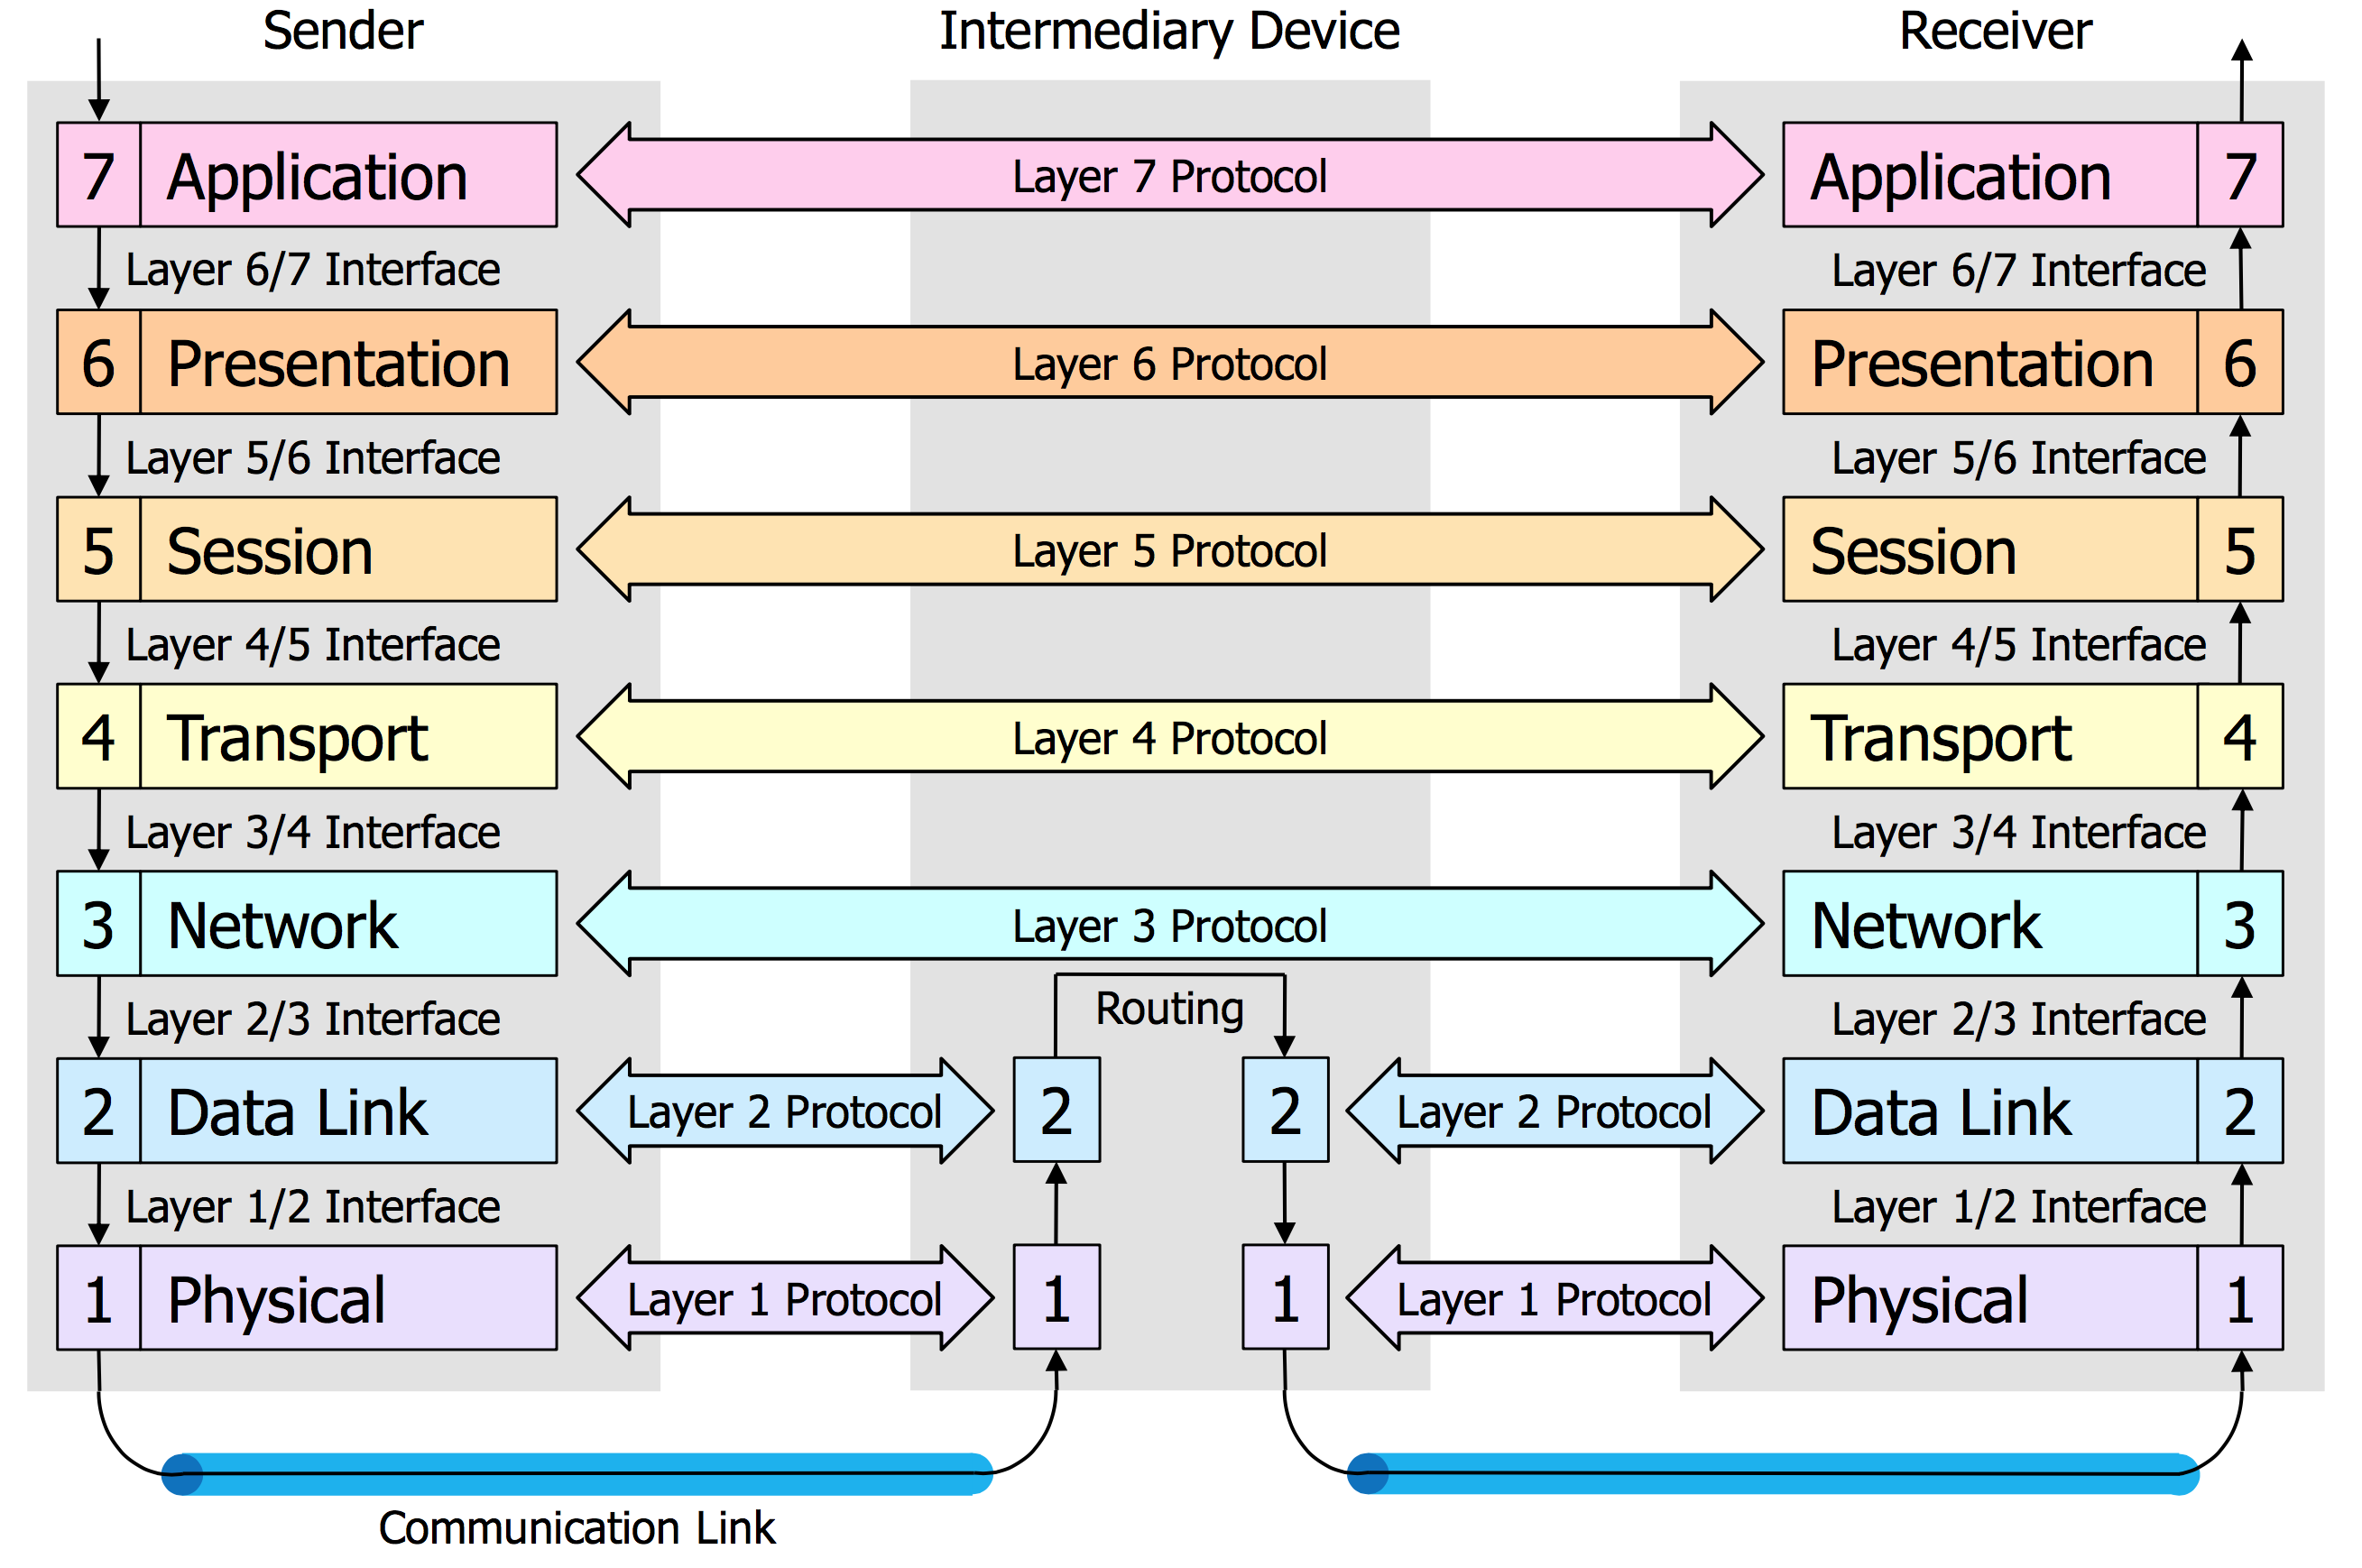
\includegraphics[trim=1 0 0 0,clip,width=\textwidth]{mainpart/analyse/img/OSI_Modell}
    \end{center}
    \caption{\ac{OSI} Referenzmodell}
\end{figure}

Für die \ac{MTU} Discovery sind vor allem die Layer 1,2,3 des \ac{OSI}-Modells\footnotemark[1] wichtig. In Layer 1 \& 2 findet die eigentliche physische Übertragung statt. So ist beispielsweise das Ethernet Protokoll sowohl im physischen Layer als auch im Data-Link-Layer vorhanden.

Die Protokolle der ersten beiden Layern haben im Vergleich zu den höheren Layern einen grossen Unterschied. Sie können nur eine begrenzt grosse Payload enthalten. So ist die maximale Payload bei Ethernet zum Beispiel 1500 Bytes. Ein Paket des Netzwerk-Layers (Layer 3) darf als maximal 1500 Bytes gross sein wenn es über Ethernet übertragen werden soll. Diese maximale Payload nennt man \acl{MTU} \acs{MTU}.

\footnotetext[1]{Bild: HSR Vorlesung CN1 - Steffen/Stettler, 29.07.2014, 1-Grundlagen.ppt}

Wenn ein Layer 3 Paket grösser als die \ac{MTU} ist dann muss es in mehrere Pakete aufgeteilt werden. Dieser Vorgang wird Fragmentierung genannt. Auch wenn Paket-Fragmentierung auftritt funktioniert eine Netzwerkverbindung normalerweise immer noch problemlos, es gibt jedoch auf Grund der Fragmentierung Performance-Einbussen. Daher versucht man, wenn möglich, Paket-Fragmentierung zu vermeiden.

\subsection{Hardware Abhängigkeit}
Die \ac{MTU} ist ein Hardware abhängiger Wert, der je nach der eingesetzten Technologie anders ist. Die Tabelle unten zeigt die \ac{MTU}s von einigen heute verwendeten Übertragungstechnologien.

\begin{table}[H]
\begin{tabularx}{\textwidth}{l|>{\raggedright\arraybackslash}X} 
\textbf{Technologie} & \textbf{MTU in Bytes} \\
\hline
\ac{FDDI} \cite[:915]{rfc1191} & 4352 \\
Ethernet \cite[:915]{rfc1191} & 1500 \\
\ac{PPPoE} \cite[:374]{rfc2516}& 1492 \\
X.25 Networks / ISDN \cite[:915]{rfc1191} & 576 \\
\end{tabularx}
\caption{Typische MTU-Grössen}
\end{table}

Wenn eine Verbindung von A nach B in mehrere Wegstrecken aufgeteilt ist und für diese Wegstrecken unterschiedliche Technologien verwendet werden dann ist die tiefste \ac{MTU} relevant für das Versenden von Paketen.

\subsection{Path MTU Discovery}
Da die \ac{MTU} bei einer neuen Verbindung noch unbekannt ist muss sie zuerst ermittelt werden. Normalerweise geschieht dies automatisch via \ac{PMTUD}. Dabei werden \ac{ICMP} Pakete unterschiedlicher Grösse die mit einem \enquote{Don't fragment} Flag versehen sind über die Verbindung gesandt. Wenn ein solches Paket auf ein Netzwerkgerät trifft dass nur eine tiefere \ac{MTU} unterstützt wird das Paket nicht weitergesendet, stattdessen wird ein \ac{ICMP} Paket mit dem Inhalt "Fragmentation needed" retourniert. So weiss der \ac{PMTUD} Algorithmus dass die \ac{MTU} der Verbindung überschritten wurde \cite[:131]{rfc1191}.

\ac{PMTUD} hat jedoch ein Problem. Router die, die \ac{ICMP} Pakete weiterleiten oder aber ein \enquote{Fragmentation needed} Paket zurücksenden sollten tun dies nicht immer. Dieses Fehlverhalten gibt es aus mehreren Gründen. Zum einen wegen Kernel-Bugs, Fehlkonfigurationen und zum anderen auch weil Firewalls manchmal so konfiguriert werden dass sie \ac{ICMP} Nachrichten nicht durchlassen auf Grund von Sicherheitsbedenken \cite[:137]{rfc2923}.

Da man sich also nicht auf \ac{PMTUD} verlassen kann um die \ac{MTU} einer Verbindung festzustellen wird mit dieser Arbeit eine \ac{MTU} Discovery implementiert die innerhalb einer \ac{IPsec} \ac{VPN} Verbindung durchgeführt werden kann.
